%% ----------------------------------------------------------------
%% Thesis.tex -- MAIN FILE (the one that you compile with LaTeX)
%% ---------------------------------------------------------------- 

% Set up the document
\documentclass[a4paper, 11pt, oneside]{Thesis}  % Use the "Thesis" style, based on the ECS Thesis style by Steve Gunn
\newcommand{\setimp}{\newif \ifimp \imptrue}
\newcommand{\unsetimp}{\newif \ifimp \impfalse}

% change the below line to \setimp to switch to implementation phase template
\unsetimp

% Include any extra LaTeX packages required
\usepackage[square, numbers, comma, sort&compress]{natbib}  % Use the "Natbib" style for the references in the Bibliography
\usepackage[nottoc]{tocbibind} % bind bibliography to the table of contents
\usepackage{verbatim}  % Needed for the "comment" environment to make LaTeX comments
\usepackage{vector}  % Allows "\bvec{}" and "\buvec{}" for "blackboard" style bold vectors in maths
\usepackage[table]{xcolor}
\hypersetup{urlcolor=black, colorlinks=true}  % Colours hyperlinks in black, can be distracting if there are many links and colored blue.
\usepackage{graphicx}
\graphicspath{{Figures/}}  % Location of the graphics files (set up for graphics to be in PDF format)

%% ----------------------------------------------------------------
\begin{document}

\frontmatter      % Begin Roman style (i, ii, iii, iv...) page numbering

% Set up the Title Page
\title  {Enhancing Accuracy in Optical Character Recognition of Sensor Readings: A Comparative Study of Tesseract and CRNN Models with Emphasis on Image Preprocessing}
\authors  {Aidan Dennehy [R00145278]}

\addresses  {\groupname\\\deptname\\\univname}  % Do not change this here, instead these must be set in the "Thesis.cls" file, please look through it instead
\date       {\today}
\subject    {}
\keywords   {}

\maketitle
%% ----------------------------------------------------------------

\setstretch{1.3}  % It is better to have smaller font and larger line spacing than the other way round

% Define the page headers using the FancyHdr package and set up for one-sided printing
\fancyhead{}  % Clears all page headers and footers
\rhead{\thepage}  % Sets the right side header to show the page number
\lhead{}  % Clears the left side page header

\pagestyle{fancy}  % Finally, use the "fancy" page style to implement the FancyHdr headers

%% ----------------------------------------------------------------
% Declaration Page required for the Thesis
\Declaration{

    \addtocontents{toc}{\vspace{1em}}  % Add a gap in the Contents, for aesthetics

    I, Aidan Dennehy , declare that this thesis titled,  "Enhancing Accuracy in Optical Character Recognition of Sensor Readings: A Comparative Study of Tesseract and CRNN Models with Emphasis on Image Preprocessing" and the work presented in it are my own. I confirm that:

    \begin{itemize}
        \item[\tiny{$\blacksquare$}] This work was done wholly or mainly while in candidature for an undergraduate degree at Munster Technological University.

        \item[\tiny{$\blacksquare$}] Where any part of this thesis has previously been submitted for a degree or any other qualification at Munster Technological University or any other institution, this has been clearly stated.

        \item[\tiny{$\blacksquare$}] Where I have consulted the published work of others, this is always clearly attributed.

        \item[\tiny{$\blacksquare$}] Where I have quoted from the work of others, the source is always given. With the exception of such quotations, this project report is entirely my own work.

        \item[\tiny{$\blacksquare$}] I have acknowledged all main sources of help.

        \item[\tiny{$\blacksquare$}] Where the thesis is based on work done by myself jointly with others, I have made clear exactly what was done by others and what I have contributed myself.
            \\
    \end{itemize}


    Signed:\\
    \rule[1em]{25em}{0.5pt}  % This prints a line for the signature

    Date:\\
    \rule[1em]{25em}{0.5pt}  % This prints a line to write the date
}
\clearpage  % Declaration ended, now start a new page

%% ----------------------------------------------------------------

% The Abstract Page
\addtotoc{Abstract}  % Add the "Abstract" page entry to the Contents
\abstract{
    \addtocontents{toc}{\vspace{1em}}  % Add a gap in the Contents, for aesthetics

    This research is primarily dedicated to the formulation of an innovative method for accurately interpreting sensor data obtained from digitized images. Confronting inherent challenges such as diminished contrast and subpar image quality, often associated with sensor readings, the study exploits Optical Character Recognition (OCR). This is accomplished employing two distinct techniques: Tesseract and Convolutional Recurrent Neural Network (CRNN) models.

    An unique feature of the research lies in its novel image preprocessing steps, specifically the masking of red and green colors prior to conversion to grayscale. This process considerably augments the efficacy of OCR. Additionally, the study underlines the critical importance of correct font selection for each sensor to enhance reading accuracy.

    The findings highlight the essential role of image quality and contrast in OCR, while presenting an innovative approach to image preprocessing for improved results. The potential implications of this research are extensive and could shape future undertakings in the fields of OCR and sensor digitization. The research underscores the vital aspects of image preprocessing and reveals how precise interventions can markedly improve sensor data interpretation from digitized images.

}

\clearpage  % Abstract ended, start a new page
%% ----------------------------------------------------------------

\setstretch{1.3}  % Reset the line-spacing to 1.3 for body text (if it has changed)

% The Acknowledgements page, for thanking everyone
\acknowledgements{
    \addtocontents{toc}{\vspace{1em}}  % Add a gap in the Contents, for aesthetics

    Acknowledgements here \ldots

}
\clearpage  % End of the Acknowledgements
%% ----------------------------------------------------------------

\pagestyle{fancy}  %The page style headers have been "empty" all this time, now use the "fancy" headers as defined before to bring them back


%% ----------------------------------------------------------------
\lhead{\emph{Contents}}  % Set the left side page header to "Contents"
\tableofcontents  % Write out the Table of Contents

%% ----------------------------------------------------------------
\lhead{\emph{List of Figures}}  % Set the left side page header to "List if Figures"
\listoffigures  % Write out the List of Figures

%% ----------------------------------------------------------------
\lhead{\emph{List of Tables}}  % Set the left side page header to "List of Tables"
\listoftables  % Write out the List of Tables

%% ----------------------------------------------------------------
\setstretch{1.5}  % Set the line spacing to 1.5, this makes the following tables easier to read
\clearpage  % Start a new page
\lhead{\emph{Abbreviations}}  % Set the left side page header to "Abbreviations"
\listofsymbols{ll}  % Include a list of Abbreviations (a table of two columns)
{
    % \textbf{Acronym} & \textbf{W}hat (it) \textbf{S}tands \textbf{F}or \\
    \textbf{LAH} & \textbf{L}ist \textbf{A}bbreviations \textbf{H}ere \\

}

%% ----------------------------------------------------------------
% End of the pre-able, contents and lists of things
% Begin the Dedication page

\setstretch{1.3}  % Return the line spacing back to 1.3

\pagestyle{empty}  % Page style needs to be empty for this page
\dedicatory{For/Dedicated to/To my\ldots}

\addtocontents{toc}{\vspace{2em}}  % Add a gap in the Contents, for aesthetics

%% ----------------------------------------------------------------
\mainmatter	  % Begin normal, numeric (1,2,3...) page numbering
\pagestyle{fancy}  % Return the page headers back to the "fancy" style

\doublespacing

\chapter{Introduction}
\label{chap:intro}
\lhead{\emph{Introduction}}


Optical Character Recognition (OCR) technology has seen substantial advancements in recent years, transforming the process of data extraction from visual mediums to digital formats. This technology, crucial in numerous fields ranging from document digitization to automated data entry systems, holds specific importance when it comes to interpreting sensor readings, a key aspect of data-driven industries. The necessity for accurate, efficient, and automated reading of sensor-generated data has led to the investigation of various techniques and models within the OCR domain.

Two models have prominently emerged as potential solutions, namely Tesseract, an open-source OCR engine sponsored by Google, and Convolutional Recurrent Neural Network (CRNN), a combination of CNN, RNN, and Connectionist Temporal Classification that offers promising results in scene text recognition tasks.

In OCR applications, image preprocessing has a pivotal role. It prepares an image for further processing by reducing noise and unnecessary details and enhancing features that are important for later stages, thereby directly influencing the accuracy of the final output. Among various preprocessing techniques, the novel approach of red and green color masking, followed by conversion to grayscale, has shown to significantly improve the accuracy of digit recognition.

In addition to these techniques, the selection of the correct font for each sensor is another critical element that affects the accuracy of the OCR system. Despite its importance, this aspect has been less emphasized in existing literature, thereby forming a crucial area of exploration in this study.

This literature review explores the current state of OCR technologies, with a particular focus on Tesseract and CRNN models. It delves into various image preprocessing techniques, emphasizing the unique method of red and green color masking before conversion to grayscale. Lastly, it investigates the role of font selection in enhancing OCR accuracy, thereby setting the context for the subsequent research.

% Putting in comments within the TeX file can be really useful in making notes for yourself and dumping text that you intend to edit later

\section{Motivation}
Why is it important to do a project on this topic? This should cover your key motivation for this. For example an excellent student from 2016 noticed a large number of homeless sleeping rough in Cork and was motivated to develop a system that load balanced the homeless shelters to try to accommodate the maximum number of homeless. This section can include the personal pronoun but the rest of the report should be third person passive, this is the case with most technical reports! For example here it is fine to say "... I decided to develop and app to help ...".

\section{Contribution}
Enumerate the main contributions. Here try to zoom out, to talk from the perspective of a Computer Science graduate. In other words, imagine you are talking to a job panel, and you want to show your computer science skills by enumerating how they are reflected in your project work. A good guide here is to look back over the modules you have covered as an undergrad from 2/3rd year, how many tools and techniques from these modules do you have in the project and to what extent? How have you advanced beyond the module content? Do you have anything new?

\section{Structure of This Document}
% notice how I cross referenced the chapters through using the \label tag --> LaTeX is VERY similar to HTML and other mark up languages so you should see nothing new here!
This section is quite formulaic. Briefly describe the structure of this document, enumerating what does each chapter and section stands for. For instance in this work in Chapter \ref{chap:background} the guidance in structuring the literature review is given. Chapter \ref{chap:problem} describes the main requirements for the problem definition and so on ... % Introduction
\chapter{Literature Review}
\label{chap:litreview}
\lhead{\emph{Literature Review}}
% \linespread{8}

% \doublespacing

\section{Introduction}

In the dynamic and continuously evolving field of computer vision and optical character recognition (OCR), two concepts have emerged as among the significant game-changers: the Tesseract OCR engine and Convolutional Recurrent Neural Networks (CRNNs). Tesseract, initially developed by Hewlett-Packard and later adopted by Google, is a pioneering engine that converts images of text into machine-encoded text, offering groundbreaking utilities across numerous applications. On the other hand, CRNNs, a deep learning-based approach, combine the spatial feature extraction capabilities of Convolutional Neural Networks (CNNs) with the sequential data processing capacity of Recurrent Neural Networks (RNNs). These networks have set new benchmarks in the realm of scene text recognition, overcoming the challenges posed by variations in text sizes, fonts, and orientations. This literature review delves into the intricacies of these advanced tools, shedding light on their principles, applications, strengths, and potential areas for improvement, thereby enriching our understanding of current trends in OCR technology and pointing to the future possibilities.


In addition to these techniques, the selection of the correct font for each sensor is another critical element that affects the accuracy of the OCR system. Despite its importance, this aspect has been less emphasized in existing literature, thereby forming a crucial area of exploration in this study.

This literature review explores the current state of OCR technologies, with a particular focus on Tesseract and CRNN models. It delves into various image preprocessing techniques, emphasizing the unique method of red and green color masking before conversion to grayscale. Lastly, it investigates the role of font selection in enhancing OCR accuracy, thereby setting the context for the subsequent research.

While this review focuses on the promising capabilities of Tesseract OCR and Convolutional Recurrent Neural Networks (CRNNs) in the OCR domain, it's crucial to acknowledge that the OCR landscape is not limited to these technologies. Many other methods play equally significant roles in expanding the OCR frontiers and opening up new avenues for research and application. Long Short-Term Memory Networks (LSTMs), Transformers, attention-based OCR models, rule-based systems, Support Vector Machines (SVMs), Hidden Markov Models (HMMs), K-Nearest Neighbors (KNN), and template matching are some of these diverse methodologies that provide unique perspectives and solutions in the OCR realm. Each of these methods has its distinctive advantages, making them optimal for certain types of tasks, as well as its limitations, requiring continuous research and development for enhancement. However, the scope of this review will mainly revolve around Tesseract and CRNNs, while the mentioned methods provide an essential context for understanding the broader OCR ecosystem.


\section{Tesseract OCR}

\section{Convolutional Recurrent Neural Networks (CRNNs)}
\newpage

\section{Other OCR Methods}

\subsection{Long Short-Term Memory Networks (LSTMs)}

Long Short-Term Memory Networks (LSTMs) are a special kind of recurrent neural network capable of learning long-term dependencies, which makes them highly suitable for OCR tasks. They've been used successfully to decode sequences of characters from images.\cite{breuelHighPerformanceOCRPrinted2013}

Breuel et al. in the paper "High-Performance OCR for Printed English and Fraktur using LSTM Networks" write about a novel application of bidirectional Long Short-Term Memory (LSTM) networks to the problem of machine-printed Latin and Fraktur recognition, without segmentation, language modelling or post-processing.

\begin{figure}[ht]
    \centering
    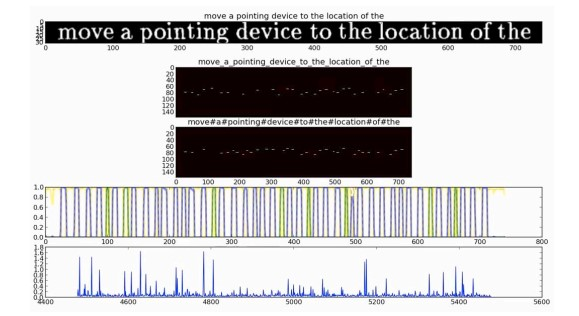
\includegraphics[width=0.8\textwidth]{Figures/LSTM_Breuel.jpg}
    \caption[Bruel's illustration of the training steps of the LSTM recognizer]{Greyscale image with background cleaning}\cite{breuelHighPerformanceOCRPrinted2013}
    \label{fig:Breuel LSTM Paper}
\end{figure}



A preprocessing step for text-line normalisation that uses a dictionary of connected component shapes and associated baseline and x-height information to map the input text lines to a fixed size output image.

A comparison of the LSTM-based system with other OCR systems on printed English and Fraktur texts, showing that LSTM achieves very low error rates and generalizes well to unseen data.

\newpage

\subsection{Transformers}

Originally developed for natural language processing tasks, Transformer models have been adapted for OCR. They treat the OCR problem as a sequence-to-sequence translation task, translating the input image into a sequence of characters.

\begin{figure}[ht]
    \centering
    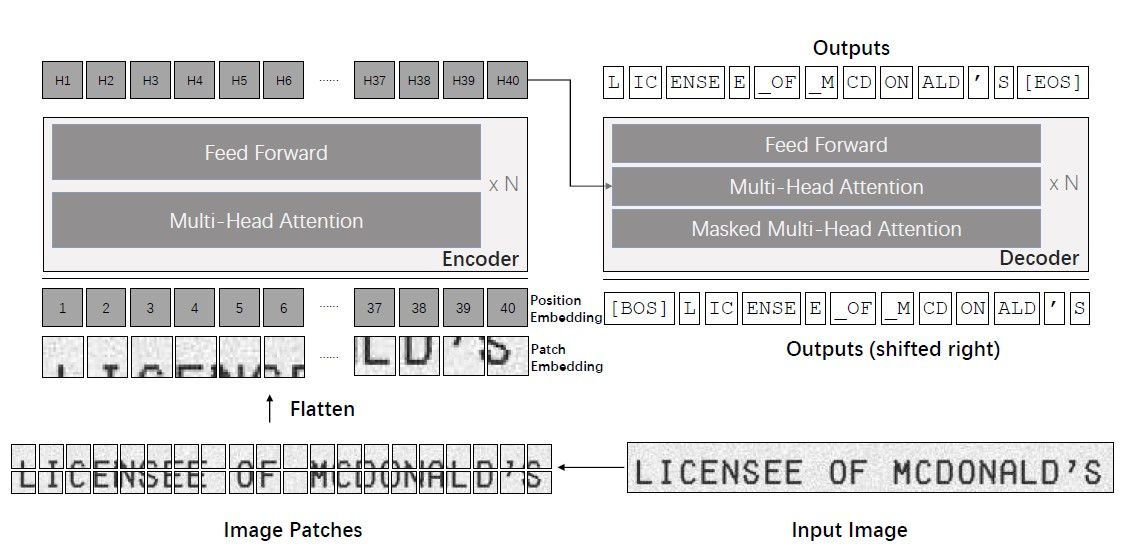
\includegraphics[width=0.6\textwidth]{Figures/Trans_MLi.jpg}
    \caption[Li's Architecture of TrOCR]{Li's Architecture of TrOCR}\cite{liTrOCRTransformerBasedOptical2023}
    \label{fig:Li's Architecture of TrOCR}
\end{figure}

M.Li et al.'s "TrOCR: Transformer-Based Optical Character Recognition with Pre-trained Models" paper proposes an end-to-end text recognition approach with pre-trained image Transformer and text Transformer models, which leverages the Transformer architecture for both image understanding and wordpiece-level text generation. \cite{liTrOCRTransformerBasedOptical2023}

Transformer based OCR models have the advantage of being able to handle long sequences of text, which is useful for OCR tasks. However, they are computationally expensive and require large amounts of training data.

CRNNs are more suitable for this project because they are faster and require less training data and are better at handling spatial information

\newpage

\subsection{Attention-based OCR models}

Attention mechanisms allow models to focus on different parts of the input image while predicting each character in the output sequence, similar to how humans read. This can improve accuracy, especially on more complex images.

Li et al.'s "Attention Based RNN Model for Document Image Quality Assessment" paper proposes a novel method for document image quality assessment (DIQA). The method integrates convolutional neural networks (CNNs) and recurrent neural networks (RNNs) to capture spatial features and attention mechanisms. It also uses reinforcement learning to train a locator network that selects the optimal regions for quality evaluation.

The CNNs are used to extract spatial features from the document images. The RNNs are used to capture the temporal dependencies between the features. The locator network is used to select the optimal regions for quality evaluation. The regions are selected based on the attention mechanism, which identifies the most important regions in the document images. \cite{liAttentionBasedRNN2017}


\begin{figure}[ht]
    \centering
    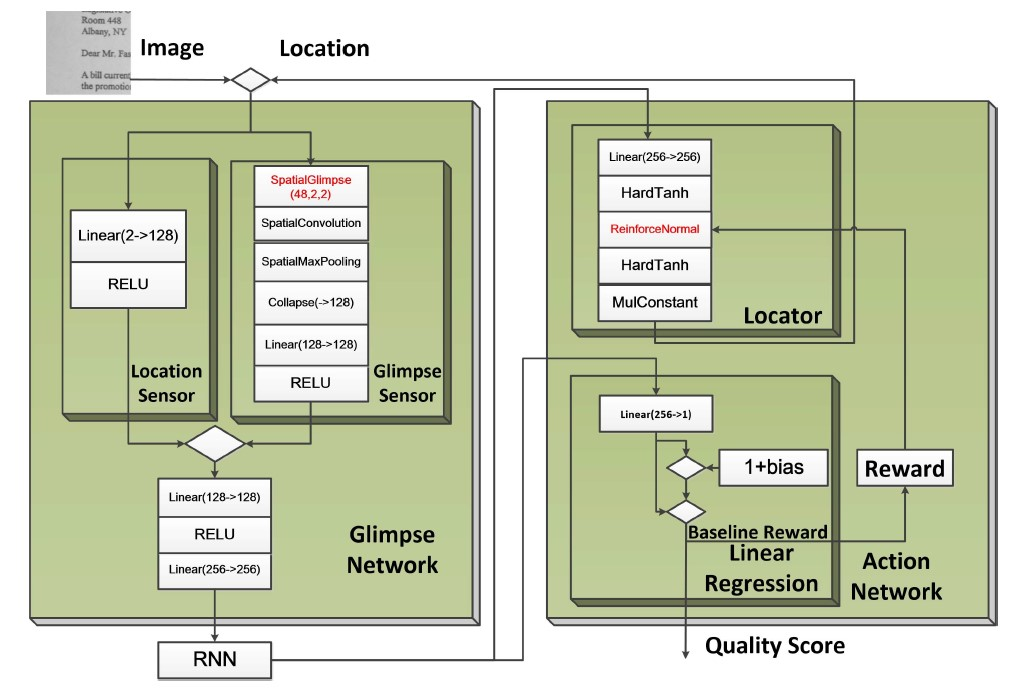
\includegraphics[width=0.6\textwidth]{Figures/AT_Li.jpg}
    \caption[Architecture of Li's proposed network]{Architecture of Li's proposed network}\cite{liAttentionBasedRNN2017}
    \label{fig:Li's Proposed Architecture}
\end{figure}

RNNs are good at handling sequential information but are poor at handling spatial information. CRNN's are more complex and combine the strengths of CNNs and RNNs which is more suitable for the this paper's OCR task.



\newpage

\subsection{Rule-based systems}

These were some of the earliest methods for OCR and use specific rules for identifying characters based on their shape, size, and relative position. They are now less commonly used due to their limitations with complex and diverse inputs.

Doush et al.'s paper "A novel Arabic OCR post-processing using rule-based and word context techniques" developed a rule-based OCR system for Arabic text that uses a combination of horizontal and vertical projections to segment characters and then classifies them based on their shape and relative position. \cite{doushNovelArabicOCR2018}



\begin{figure}[ht]
    \centering
    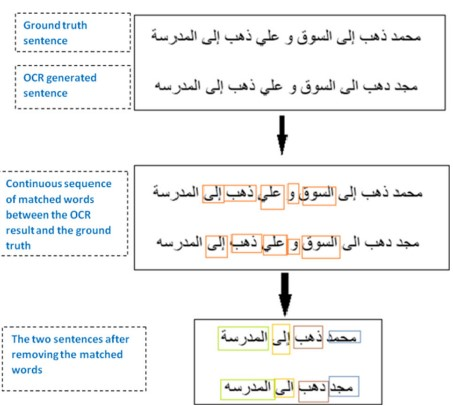
\includegraphics[width=0.6\textwidth]{Figures/RB_Doush.jpg}
    \caption[Example of applying the Rule Based FAHTA Algorithm]{Example of applying the Rule Based FAHTA Algorithm}\cite{doushNovelArabicOCR2018}
    \label{fig:Doush Rule Based OCR Paper}
\end{figure}

The FAHTA algorithm is a novel alignment technique that is used to match the ground truth text with the OCR misrecognized text. The paper also says that the FAHTA algorithm is fast, accurate, and can handle different types of OCR errors, such as over-segmentation, under-segmentation, and merging words. The paper claims that the FAHTA algorithm can be used for other languages as well.


For the purposes of this project, the rule-based system is not suitable because it requires a large number of rules to be defined for each character, which is not feasible for the large range iof digit fonts.


\newpage

\subsection{Support Vector Machines (SVMs)}

Support Vector Machines (SVMs) are used for character recognition in OCR due to their effective high-dimensional mapping and classification abilities. They work best when text is clearly segmented. In the their paper "Development of an Image Processing Techniques for Vehicle Classification Using OCR and SVM", Joshua et al. used SVMs to classify characters in a license plate image and achieved an accuracy of 98.3\% using a local dataset of 10,000 images.\cite{joshuaDevelopmentImageProcessing2023}

\begin{figure}[ht]
    \centering
    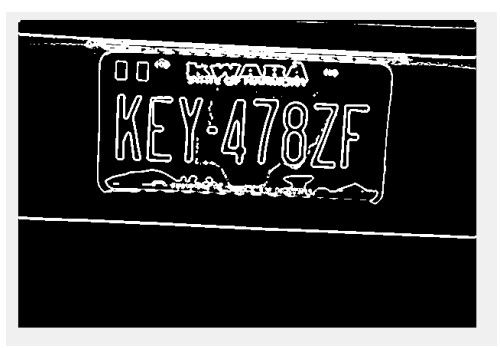
\includegraphics[width=0.8\textwidth]{Figures/SVM_Joshua.jpg}
    \caption[Development of an Image Processing Technique for Vehicle Classification using OCR and SVM]{Greyscale image with background cleaning}\cite{joshuaDevelopmentImageProcessing2023}
    \label{fig:Joshua SVM Paper}
\end{figure}

Joshua et al. describe the steps of their proposed system, which include image preprocessing, feature extraction, OCR, and SVM classification. They also explain how they collected and labeled their dataset of Nigerian vehicle plate numbers.

\newpage

\subsection{Hidden Markov Models (HMMs)}

HMMs have been used in OCR for recognizing sequential data. HMMs are statistical models that assume an underlying process to be a Markov process with hidden states.


In Rashid et al.'s "An evaluation of HMM-based Techniques for the Recognition of Screen Rendered Text" paper, they evaluate Hidden Markov Model (HMM) techniques for optical character recognition (OCR) of low resolution text from screen images and compares them with other OCR systems.

The paper uses two data sets of screen rendered characters and text-lines, and extracts two types of features from them: gray scale raw pixel features and gradient based gray level intensity features.


\begin{figure}[!h]
    \centering
    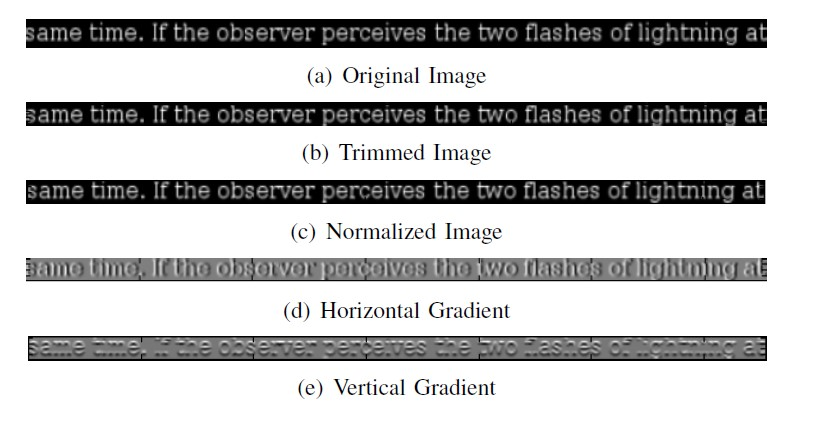
\includegraphics[width=0.8\textwidth]{Figures/HMM_Rashid.jpg}
    \caption[Rashid's Extraction steps from screen rendered text-lines]{Rashid's Extraction steps from screen rendered text-lines}\cite{rashidEvaluationHMMBasedTechniques2011}
    \label{fig:Rashid Feature Extraction Steps}
\end{figure}

The paper reports the character recognition accuracy of the HMM-based methods and other OCR engines on the two data sets. It shows that the HMM-based methods reach the performance of other methods on screen rendered text and achieve above 98\% accuracy.\cite{rashidEvaluationHMMBasedTechniques2011}

HMMs are a good choice for tasks where simplicity and interpretability are important. CRNNs are a good choice for tasks where accuracy is more important, and where the sequences are long or complex.

\newpage

\subsection{K-Nearest Neighbors (KNN)}

KNN is a simple, instance-based learning algorithm used for OCR, particularly for isolated character recognition. Hazra et al. develop an optical character recognition (OCR) system that uses a custom image to train a k-nearest neighbor (KNN) classifier. They claim that their system can recognize handwritten or printed text in any language by changing the training image and labels. \cite{hazraOpticalCharacterRecognition2017}

\begin{figure}[!h]
    \centering
    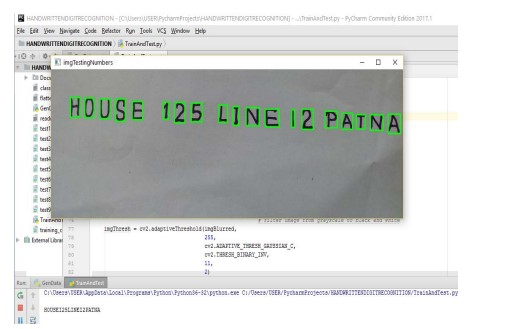
\includegraphics[width=0.8\textwidth]{Figures/KNN_Hazra.jpg}
    \caption[Optical Character Recognition using KNN on Custom
        Image Dataset]{Characters and Digits regocnised}\cite{joshuaDevelopmentImageProcessing2023}
    \label{fig:Hazra OCR KNN Paper}
\end{figure}

Hazra et al. explain the steps of their algorithm, which include image processing, feature extraction, and KNN classification. They also discuss the advantages of KNN over other classification methods, such as ease of interpretation, low computation time, and high predictive power. In this paper the authors started with clear images of known fonts, which is not the case in this project.


\newpage

\subsection{Template Matching}

Template Matching is a technique used to locate small-parts of the bigger image which match a template image. This can be useful in OCR when the set of possible characters is known and limited. In Hossain et al.'s "Optical Character Recognition based on Template Matching" paper, they use template matching to recognize characters in a license plate image.

\begin{figure}[ht]
    \centering
    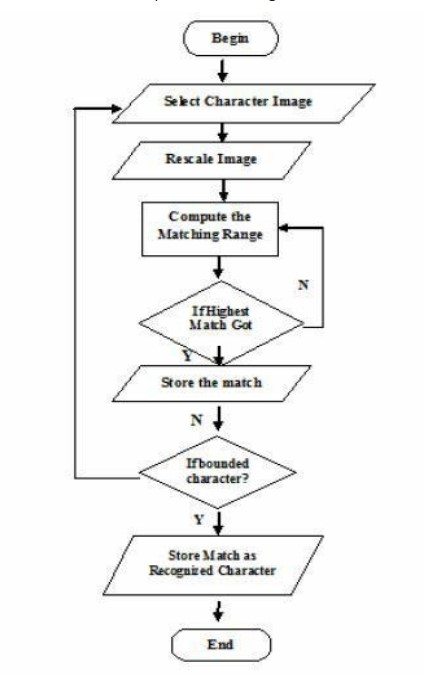
\includegraphics[width=0.4\textwidth]{Figures/TM_Hossain.jpg}
    \caption[Flowchart of Template Matching OCR]{Flowchart of Hossain's TM OCR}\cite{hossainOpticalCharacterRecognition2019}
    \label{fig:Hossain OCR Template Matching Paper}
\end{figure}

Their system prototype was tested on different text images with different fonts and sizes. The accuracy was calculated based on the character recognition accuracy. Their results show that Calibri and Verdana fonts had the highest accuracy, while Cambria and Times New Roman fonts had the lowest accuracy.  The accuracy can be improved by training the system with more fonts and features. \cite{hossainOpticalCharacterRecognition2019}


 % Literature Review 
\chapter{Methodology}
\label{chap:methodology}
\lhead{\emph{Problem Statement}}



\section{Introduction}



This chapter provides a comprehensive and detailed explanation of the techniques and procedures adopted during the course of the research. It serves to provide an in-depth account of the methods used in this study, thereby ensuring the research's transparency and reproducibility.

This research aims to enhance the performance of Optical Character Recognition (OCR) systems - specifically Tesseract OCR and Convolutional Recurrent Neural Network (CRNN) models - on images of sensor readings. To accomplish this, a systematic approach is adopted involving an initial global run of the OCR systems on the raw image datasets, followed by the application of specific image pre-processing techniques and subsequent localized OCR applications.

The purpose of these processes is to establish a baseline of OCR performance, then test the hypothesis that image pre-processing can enhance OCR results. The pre-processing, focused on applying colour masks before converting the images to grayscale, aims to increase the clarity of the images, thereby increasing the efficiency of the OCR processes.

This chapter outlines each of these processes in detail, thereby providing a clear roadmap of the research methodology adopted in this study. From the initial assessment of the OCR systems' performance to the implementation of the pre-processing techniques, this chapter serves as a guide to understanding the practical steps taken during this research project.

The subsequent sections provide further detail on the data being used, the OCR systems of focus, the pre-processing techniques applied, and the methods of evaluation. The goal of this chapter is to present a detailed and comprehensive account of the methodology that underpins this research.

---


\section{Data Collection}

The dataset used in this research was supplied as a collection of image files distributed across ten distinct folders. Each folder corresponds to a unique sensor from which readings were taken. These images provide a diversified dataset due to variations in sensor specifications and the conditions under which the readings were captured.

Upon receiving the data, an initial examination was carried out to ensure the integrity and completeness of the files. The image files were found to be in good condition, readable, and ready for further processing and analysis.

In order to streamline the data management and analysis process, a CSV file was created. This file serves as an inventory, containing each image file name and its corresponding label, thereby facilitating an efficient cross-referencing system for the data analysis phase.

To facilitate the training of the Convolutional Recurrent Neural Network (CRNN) models, multiple training databases were created. Each of these databases consists of 500,000 single digit training images, thereby providing a robust foundation for the machine learning tasks.

\newpage
\section{Data Analysis}

For each folder, there are three charts that provide an initial statistical data analysis of the images. These charts are as follows:


\begin{enumerate}
    \item \textbf{Montage:} A simple representation of the images in the folder, arranged in a grid format. This provides a visual overview of the images in the folder, thereby facilitating a quick assessment of the data.
    \item \textbf{RGB Histogram:} This chart shows the distribution of pixel intensities for the Red, Green, and Blue channels separately in each image.
          \begin{enumerate}

              \item \textit{Axes:} The X-axis represents the possible pixel intensity values (ranging from 0 to 255 for an 8-bit image), and the Y-axis represents the number of pixels in the image with that intensity value.
              \item \textit{Colour Lines:} The Red line shows the distribution of red pixel intensities, the Green line shows the distribution of green pixel intensities, and the Blue line shows the distribution of blue pixel intensities.
              \item \textit{Interpretation:} Peaks in the graph represent the colours that are most present in the image. For instance, a high peak in the red line around the value 200 would indicate that the image has many pixels with high red intensity, suggesting the image may visually appear reddish.
              \item \textit{Colour Composition:} The overall shape of these colour distributions can provide an idea about the colour composition of the images.
              \item \textit{Utility:} The RGB Histogram aids in understanding the dominant colours in the image, the contrast, and the brightness. Variations in these histograms across the image set might be related to different sensor readings or variations in image capture settings.
          \end{enumerate}
    \item \textbf{Data Analysis:} Eight metrics have been defined to quantify various properties of an image. Each of these metrics provides insight into different aspects of the image, allowing for a detailed analysis and comparison of images. These metrics are as follows:
          \begin{enumerate}

              \item \textbf{Contrast:} The Contrast chart visualizes the degree of local variation in an image, which can be associated with the details or changes in sensor readings.
              \item \textbf{Dissimilarity:} Dissimilarity, like contrast, measures local variations, offering additional information about changes in the image.
              \item \textbf{Homogeneity:} The Homogeneity chart shows the closeness of the distribution of elements in an image to its diagonal, providing insight into the uniformity or variation in sensor readings.
              \item \textbf{Energy:} The Energy chart encapsulates the sum of squared elements in the image, which can suggest patterns or randomness in sensor readings.
              \item \textbf{Correlation:} The Correlation chart illustrates the joint probability occurrence of specific pixel pairs, thereby hinting at the predictability or scatter of sensor readings.
              \item \textbf{Area:} The Area chart, in our context, represents the total area of contours detected in an image, providing information on the complexity of sensor readings.
              \item \textbf{Brightness:} The Brightness chart displays the average lightness or darkness of each image, which might be influenced by different environmental conditions or sensor settings.
              \item \textbf{Standard Deviation:} The Standard Deviation chart shows the variability in pixel intensities within each image, helping infer the contrast, detail, and complexity of sensor readings.
          \end{enumerate}


\end{enumerate}

\subsection{Folders}
\subsubsection{Sipa 2}


\begin{figure}[ht]
    \begin{subfigure}
        \centering
        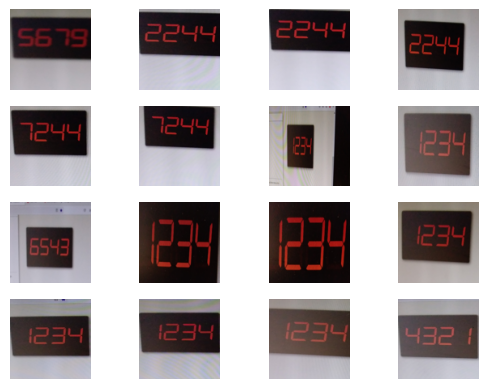
\includegraphics[width=\linewidth]{Figures/EDA_Charts/2/montage.png}
        \caption{Caption for first image}
        \label{fig:sub1}
    \end{subfigure}\hfill
    \begin{subfigure}
        \centering
        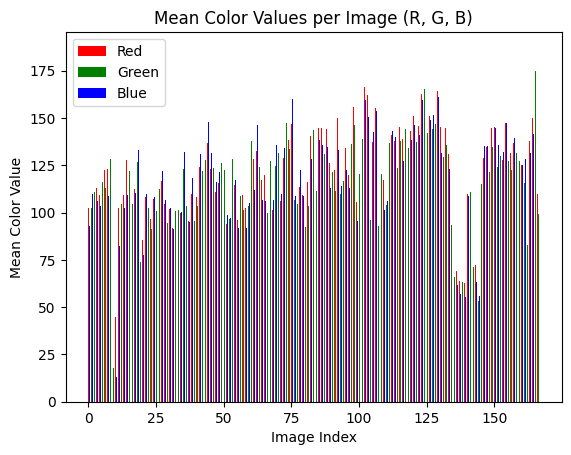
\includegraphics[width=\linewidth]{Figures/EDA_Charts/2/rgb.png}
        \caption{Caption for second image}
        \label{fig:sub2}
    \end{subfigure}\hfill
    \begin{subfigure}
        \centering
        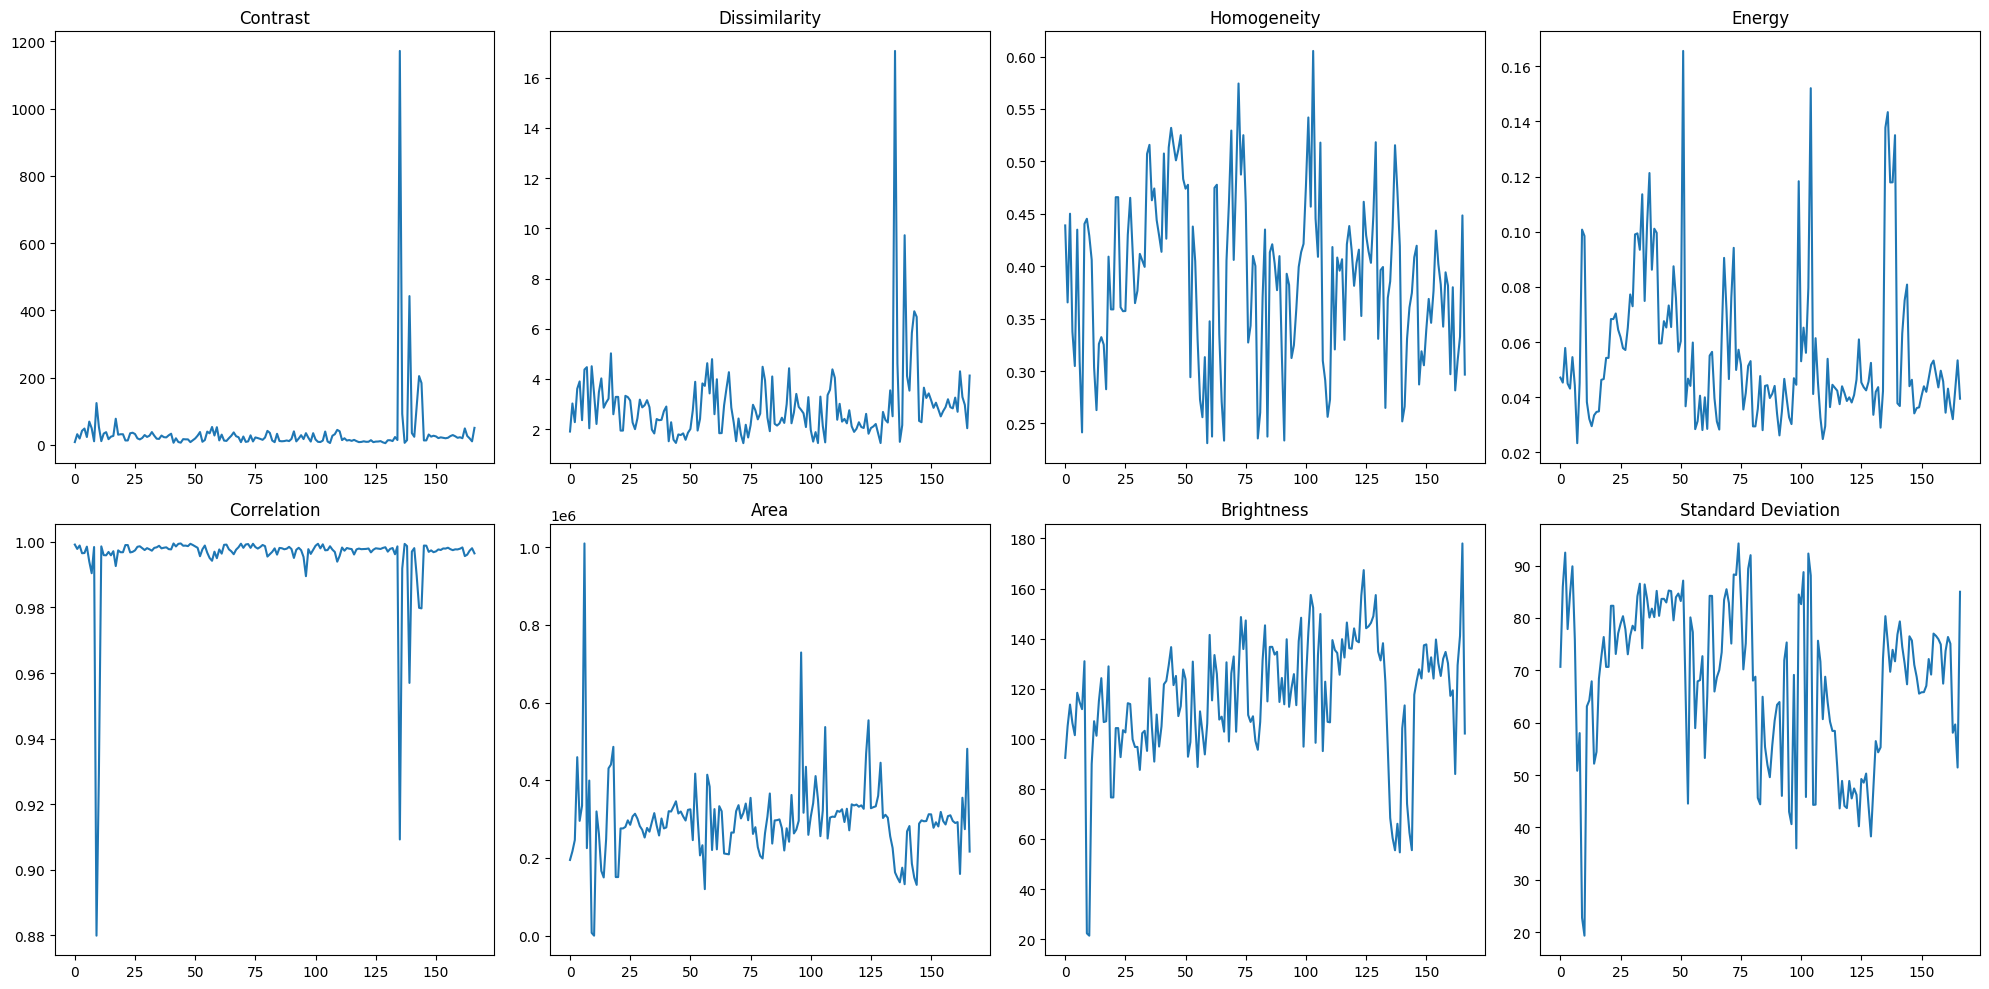
\includegraphics[width=\linewidth]{Figures/EDA_Charts/2/da.png}
        \caption{Caption for third image}
        \label{fig:sub3}
    \end{subfigure}
    \caption{Caption for whole figure}
    \label{fig:test}
\end{figure}


\begin{lstlisting}[language=Python, caption=Python example]
    def hello_world():
    print("Hello, world!")
\end{lstlisting}


the above code is a python code snippet. % Methodology
\chapter{Results}
\label{chap:results}
\lhead{\emph{Results}}

\section{Introduction} % Results
\chapter{Discussion and Conclusion}
\label{chap:conclusion}
\lhead{\emph{Discussion and Conclusion}}

\section{Introduction}

Briefly reintroduce the research's objectives and the methodologies employed.





\section{Discussion of Findings}
\subsection{OCR Performance}

Discuss the overall performance of the Tesseract OCR system on the raw image datasets.
Highlight the improvements observed after implementing the various pre-processing techniques.
Contrast the results between different image folders, noting any significant variations.

\subsection{Image Pre-processing Techniques}

Delve into the significance of each pre-processing technique:



Colour masks (Red and Green masks)
Grayscale conversion
Resizing
Thresholding techniques
Denoising
Deblurring
Others
Discuss the specific impact of each technique on OCR performance and any trade-offs observed.

\subsection{CRNN Model Analysis}

Discuss the benefits and challenges of using the CRNN model.
Contrast its performance with the Tesseract OCR system.

\section{Challenges and Limitations}

Detail any challenges faced during the research, e.g., images with diverse properties, environmental conditions affecting image quality, etc.
Discuss limitations in the methodologies used and potential areas for improvement.


\section{Implications and Applications}

Discuss the broader implications of your findings. How do they contribute to the field of OCR or specific applications like reading sensor data?
Mention potential real-world applications and benefits.
\section{Conclusions}

Summarize the main findings of your research.
Reiterate the significance of your research in enhancing the performance of OCR systems.


\section{Recommendations and Future Work}

Provide recommendations based on your findings, especially for researchers or practitioners aiming to utilize OCR for similar applications.
Discuss potential areas of future research or further enhancements that could be explored.




 % Discussion and Conclusion

%% ----------------------------------------------------------------
\label{Bibliography}

%\singlespacing
\setstretch{0.7}


\bibliographystyle{IEEEtranN}  % Use the "IEEE Transaction" BibTeX style for formatting the Bibliography
\bibliography{Bibliography}  % The references (bibliography) information are stored in the file named "Bibliography.bib"
\lhead{\emph{Bibliography}}  % Change the left side page header to "Bibliography"

%% ----------------------------------------------------------------
% Now begin the Appendices, including them as separate files

\addtocontents{toc}{\vspace{2em}} % Add a gap in the Contents, for aesthetics

\appendix % Cue to tell LaTeX that the following 'chapters' are Appendices

\chapter{Appendix A}
\lhead{\emph{Appendix A}}

\section{Introduction}

Appendix Introduction

The appendix of this thesis provides a more detailed look at the technical aspects of the research presented in the main body. This includes supporting charts, visualizations, and code snippets that explain the specific pre-processing steps, Optical Character Recognition (OCR) techniques, and font selection choices that were made.

The materials in this appendix are not essential for understanding the main findings of the thesis, but they are important for readers who want a deeper understanding of the methods and processes used. This is especially true for the novel pre-processing steps and the role of image quality and contrast in OCR.

By navigating through this appendix, enthusiasts and specialists alike will gain a deeper understanding of the intricacies that have contributed to the efficacy of the OCR approach undertaken in this Thesis.

\newpage

\section{Analysis Tesseract Separate Folders}

\subsection{Image Folder A Best Image Size Analysis}

\begin{figure}[ht]
    \centering
    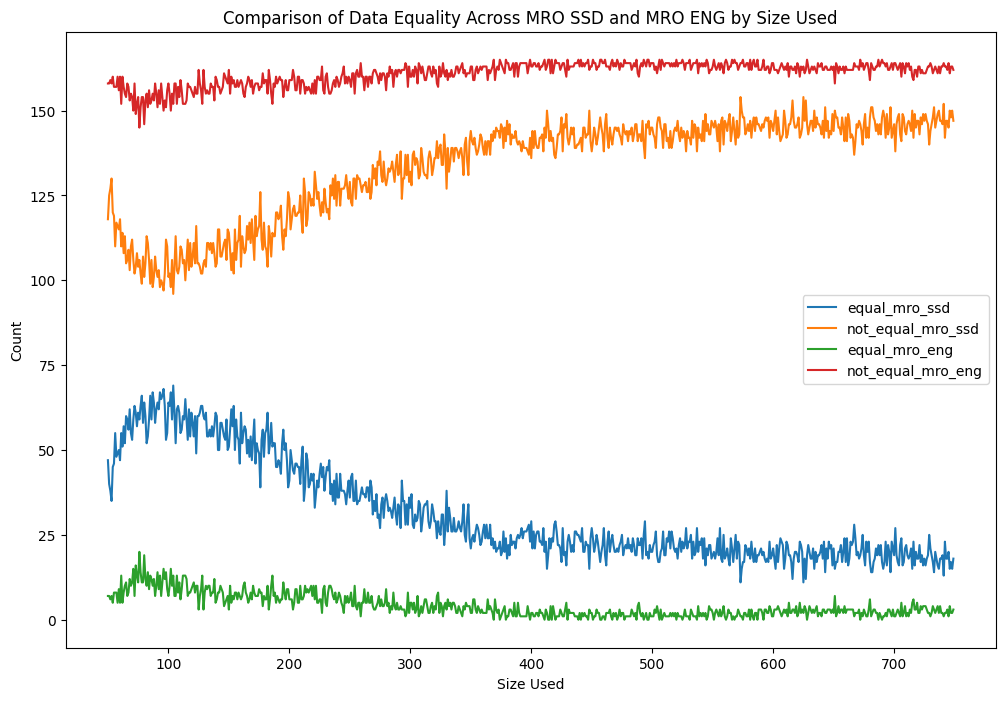
\includegraphics[width=0.9\textwidth]{Figures/Results/sipa_02/count_analysis.png}
    \caption[Count Analysis]{Image Folder A Count Analysis}
    \label{fig:Image Folder A Best Image Size Analysis}
\end{figure}

The chart presented primarily emphasizes the blue line, which signifies the count of Masked Red OTSU. This line is of particular importance. At size 104, we observe the peak read count.

This establishes the dimensions to which the images will be resized for each of the subsequent directories.

\newpage




\newpage

\subsection{Image Folder A Contrast Analysis on MRO SSD}

\begin{figure}[ht]
    \centering
    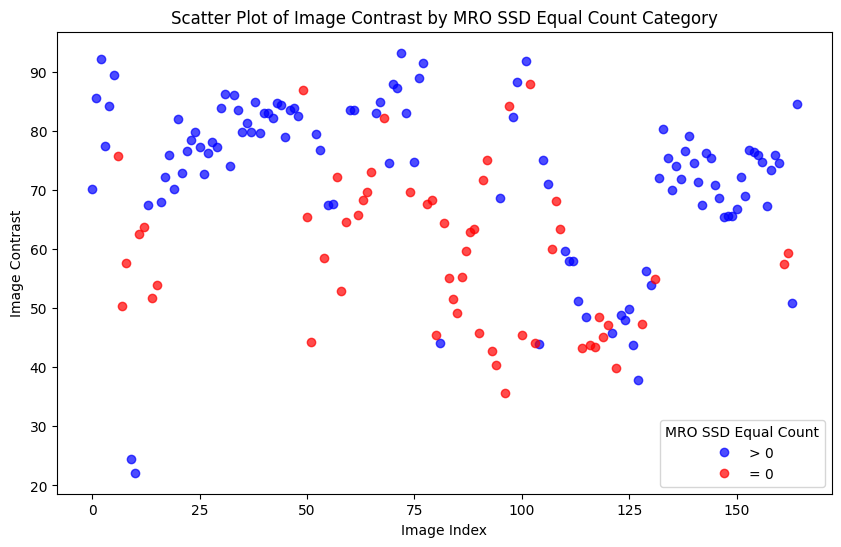
\includegraphics[width=0.9\textwidth]{Figures/Results/sipa_02/contrast.png}
    \caption[Image Folder A Contrast Analysis on MRO SSD]{Image Folder A Contrast Analysis on MRO SSD}
    \label{fig:Image Folder A Contrast Analysis on MRO SSD}
\end{figure}

The scatter plot of image contrast shows that there is a wide range of contrast levels for both categories of images (MRO SSD EQUAL COUNT greater than 0 and equal to 0). This means that the contrast of images in both categories is highly variable. Additionally, there is significant overlap in the contrast values of both categories, suggesting that the contrast of an image may not be a strong indicator of whether the MRO SSD EQUAL COUNT is greater than 0 or not.

There are a few outliers in the MRO SSD EQUAL COUNT greater than 0 category with particularly high contrast levels. However, these outliers do not significantly change the overall pattern of the scatter plot.

In summary, the scatter plot of image contrast does not provide any clear evidence that the contrast of an image is a good predictor of the MRO SSD EQUAL COUNT value.

\newpage

\subsection{Image Folder A Brightness Analysis on MRO SSD}


\begin{figure}[ht]
    \centering
    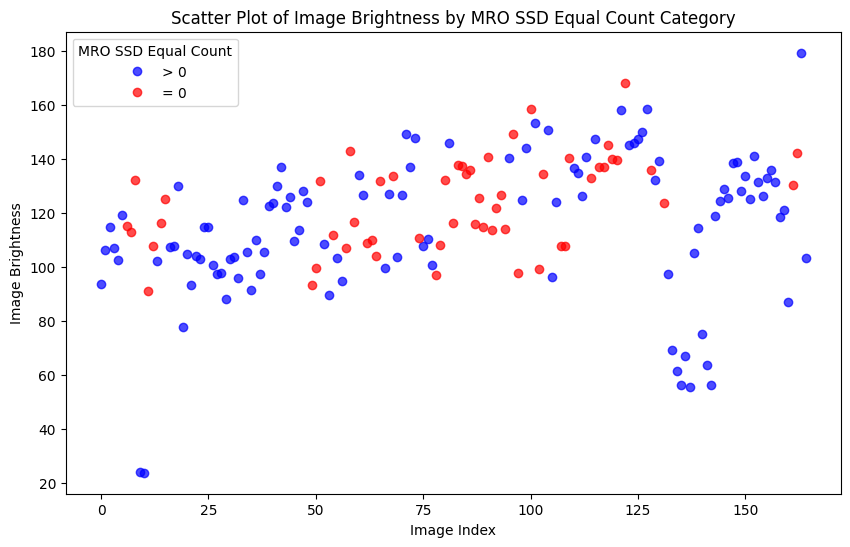
\includegraphics[width=0.9\textwidth]{Figures/Results/sipa_02/brightness.png}
    \caption[Image Folder A Brightness Analysis on MRO SSD]{Image Folder A Brightness Analysis on MRO SSD}
    \label{fig:Image Folder A Brightness Analysis on MRO SSD}
\end{figure}



The scatter plot of image brightness shows that both categories of images (MRO SSD EQUAL COUNT greater than 0 and equal to 0) have a wide range of brightness values. This means that the brightness of images in both categories is highly variable. Additionally, there is no clear pattern or correlation between the MRO SSD EQUAL COUNT category and the brightness of the images. This suggests that the brightness of an image may not be a good predictor of whether the MRO SSD EQUAL COUNT is greater than 0 or not.

There are a few outliers in the MRO SSD EQUAL COUNT greater than 0 category with particularly high brightness levels. However, these outliers do not significantly change the overall pattern of the scatter plot.

In summary, the scatter plot of image brightness does not provide any clear evidence that the brightness of an image is a good predictor of the MRO SSD EQUAL COUNT value.

\newpage

\subsection{Image Folder A Standard Deviation Analysis on MRO SSD}


\begin{figure}[ht]
    \centering
    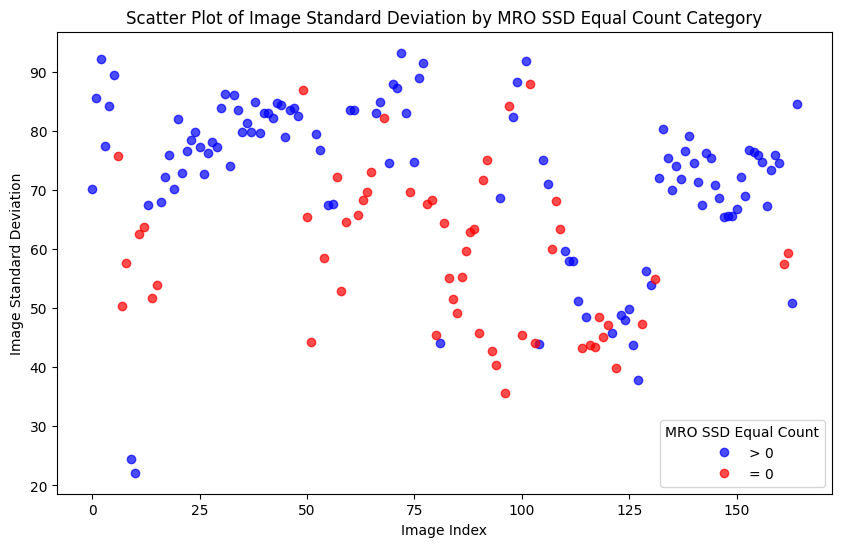
\includegraphics[width=0.9\textwidth]{Figures/Results/sipa_02/sd.png}
    \caption[Image Folder A Standard Deviation Analysis on MRO SSD]{Image Folder A Standard Deviation Analysis on MRO SSD}
    \label{fig:Image Folder A Standard Deviation Analysis on MRO SSD}
\end{figure}

The scatter plot of image standard deviation shows that there is a wide range of standard deviations for both categories of images (MRO SSD EQUAL COUNT greater than 0 and equal to 0). This means that the spread of pixel values within the images is highly variable. Additionally, there is significant overlap in the standard deviation values of both categories, suggesting that the standard deviation of pixel values within an image may not be a strong indicator of whether the MRO SSD EQUAL COUNT is greater than 0 or not.


\newpage

\subsection{Image Folder A Homogeneity Analysis on MRO SSD}


\begin{figure}[ht]
    \centering
    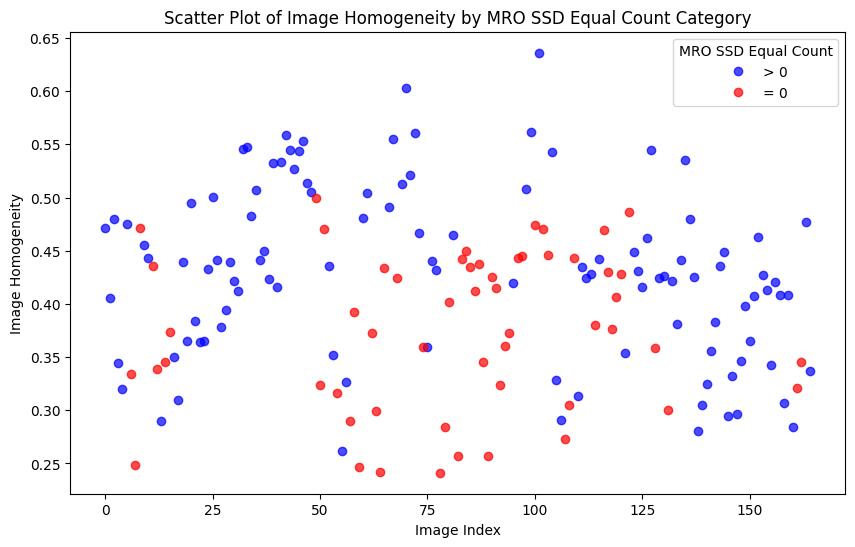
\includegraphics[width=0.9\textwidth]{Figures/Results/sipa_02/homogeneity.png}
    \caption[Image Folder A Homogeneity Analysis on MRO SSD]{Image Folder A Homogeneity Analysis on MRO SSD}
    \label{fig:Image Folder A Homogeneity Analysis on MRO SSD}
\end{figure}


The scatter plot of image Homogeneity shows that there is a wide range of homogeneity levels for both categories of images (MRO SSD EQUAL COUNT greater than 0 and equal to 0). This signifies that the homogeneity of images in both categories is highly variable. Additionally, there is significant overlap in the homogeneity values of both categories, suggesting that the homogeneity of an image may not be a strong indicator of whether the MRO SSD EQUAL COUNT is greater than 0 or not.



In summary, the scatter plot of image homogeneity does not provide any clear evidence that the homogeneity of an image is a good predictor of the MRO SSD EQUAL COUNT value.

\newpage

\subsection{Image Folder A Sharpness Analysis on MRO SSD}


\begin{figure}[ht]
    \centering
    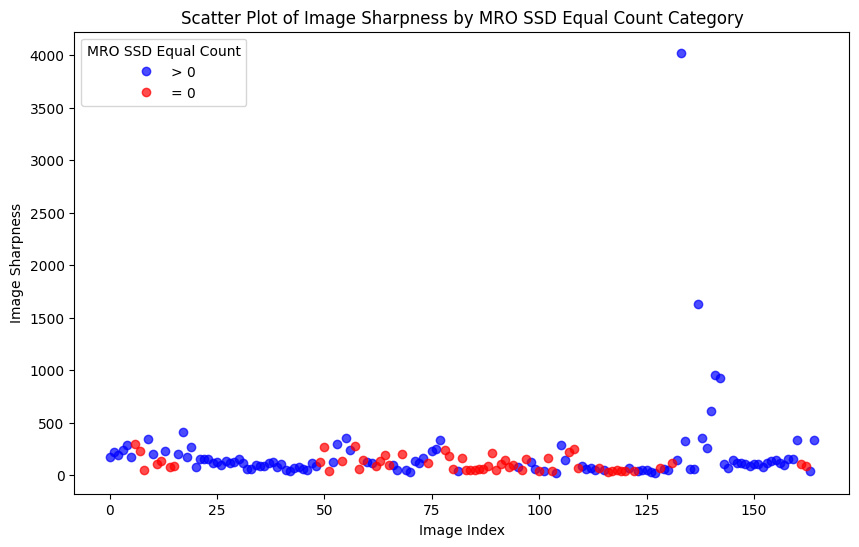
\includegraphics[width=0.9\textwidth]{Figures/Results/sipa_02/sharpness.png}
    \caption[Image Folder A Sharpness Analysis on MRO SSD]{Image Folder A Sharpness Analysis on MRO SSD}
    \label{fig:Image Folder A Sharpness Analysis on MRO SSD}
\end{figure}



The scatter plot of image Sharpness shows that there is a narrow range of sharpness levels for both categories of images (MRO SSD EQUAL COUNT greater than 0 and equal to 0). This signifies that the sharpness of images in both categories is reasonably uniform. Additionally, there is significant overlap in the sharpness values of both categories, suggesting that the sharpness of an image may not be a strong indicator of whether the MRO SSD EQUAL COUNT is greater than 0 or not.

In summary, the scatter plot of image sharpness does not provide any clear evidence that the sharpness of an image is a good predictor of the MRO SSD EQUAL COUNT value.

\newpage


\subsection{Image Folder A Dissimilarity Analysis on MRO SSD}


\begin{figure}[ht]
    \centering
    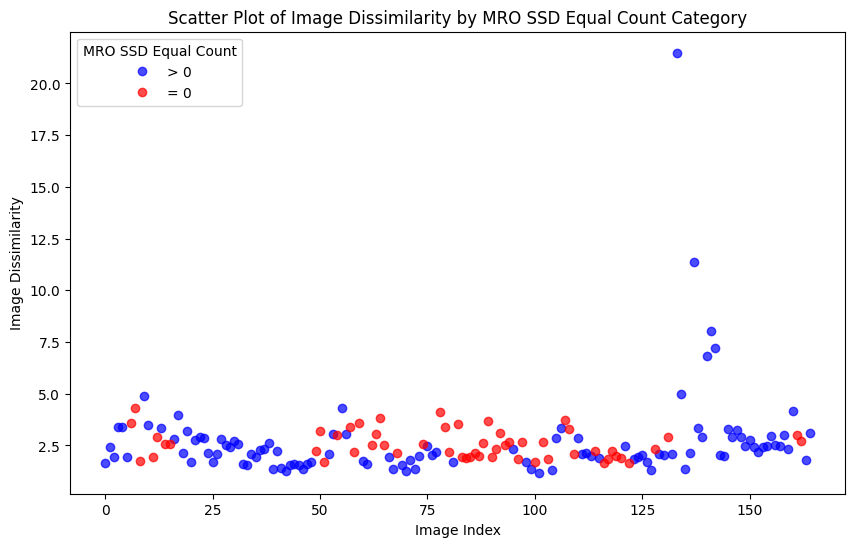
\includegraphics[width=0.9\textwidth]{Figures/Results/sipa_02/dissimilarity.png}
    \caption[Image Folder A Dissimilarity Analysis on MRO SSD]{Image Folder A Dissimilarity Analysis on MRO SSD}
    \label{fig:Image Folder A Dissimilarity Analysis on MRO SSD}
\end{figure}



The scatter plot of image Dissimilarity shows that there is a narrow range of dissimilarity levels for both categories of images (MRO SSD EQUAL COUNT greater than 0 and equal to 0). This signifies that the dissimilarity of images in both categories is reasonably uniform. Additionally, there is significant overlap in the dissimilarity values of both categories, suggesting that the dissimilarity of an image may not be a strong indicator of whether the MRO SSD EQUAL COUNT is greater than 0 or not.

In summary, the scatter plot of image dissimilarity does not provide any clear evidence that the dissimilarity of an image is a good predictor of the MRO SSD EQUAL COUNT value.


\newpage

\subsection{Image Folder A Area Analysis on MRO SSD}


\begin{figure}[ht]
    \centering
    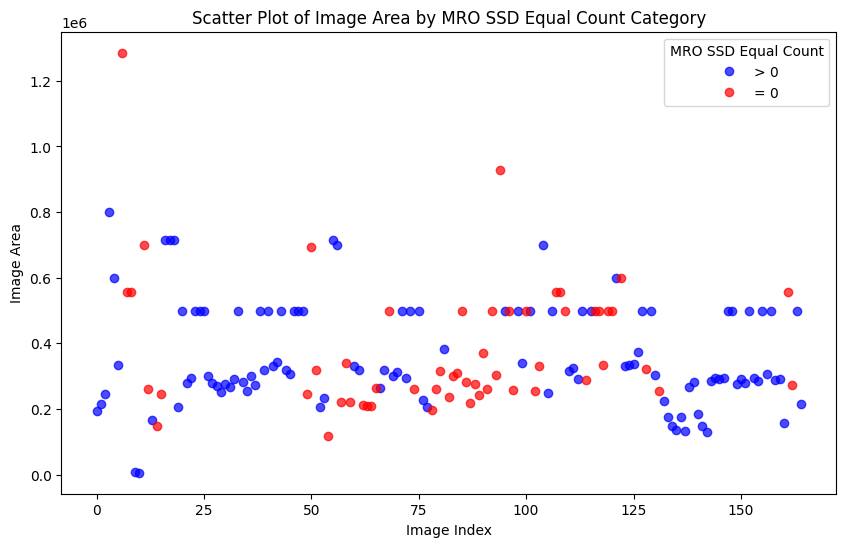
\includegraphics[width=0.9\textwidth]{Figures/Results/sipa_02/area.png}
    \caption[Image Folder A Area Analysis on MRO SSD]{Image Folder A Area Analysis on MRO SSD}
    \label{fig:Image Folder A Area Analysis on MRO SSD}
\end{figure}


The distribution of image area values for both categories (> 0 and = 0) is wide. However, the distribution appears to be slightly different for the two categories, with a higher density of points at lower image area values for the = 0 category.

There is a significant density of points near the lower end of the image area values for both categories. The = 0 category seems to have a higher density of points at lower image area values.

There is considerable overlap between the two categories, especially at lower image area values. This suggests that while there may be a trend, the MRO SSD EQUAL COUNT value is not a definitive predictor of the image area value.

There appear to be some outliers in the >0 category with high image area values. This suggests that there may be some instances where MRO SSD EQUAL COUNT is greater than 0 and the image area is significantly larger than the typical values.

In summary, this scatter plot suggests that there might be a slight tendency for instances with MRO SSD EQUAL COUNT of 0 to have smaller image areas. However, the relationship is not clear-cut, as there is significant overlap between the two categories.



\newpage

\subsection{Image Folder A Correlation Analysis on MRO SSD}


\begin{figure}[ht]
    \centering
    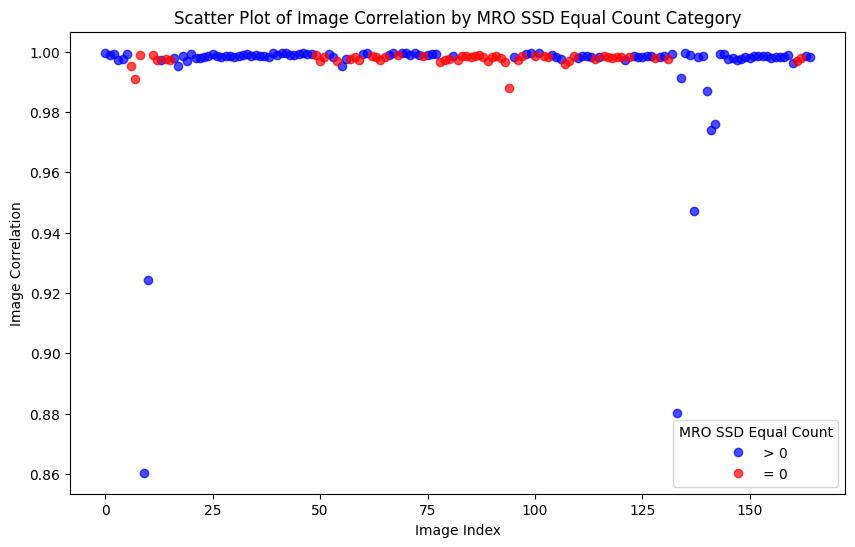
\includegraphics[width=0.9\textwidth]{Figures/Results/sipa_02/correlation.png}
    \caption[Image Folder A Correlation Analysis on MRO SSD]{Image Folder A Correlation Analysis on MRO SSD}
    \label{fig:Image Folder A Correlation Analysis on MRO SSD}
\end{figure}

The distribution of image correlation values for both categories (> 0 and = 0) is varied, similar to the previous plot.

The density of points for both categories appears to be quite uniform across the range of image correlation values. There is perhaps a slightly higher density at lower correlation values for the = 0 category.

There is significant overlap between the two categories across the entire range of image correlation values. This suggests that the MRO SSD EQUAL COUNT value does not strongly distinguish between different levels of image correlation.

There do not seem to be any clear outliers in this plot, unlike the previous plot for Image Energy.

In summary, while there might be a slight tendency for instances with MRO SSD EQUAL COUNT of 0 to have lower image correlation, the relationship is not clear-cut. There is substantial overlap between the two categories, indicating that MRO SSD EQUAL COUNT may not be a strong predictor for image correlation.

\newpage

\subsection{Image Folder A Energy Analysis on MRO SSD}


\begin{figure}[ht]
    \centering
    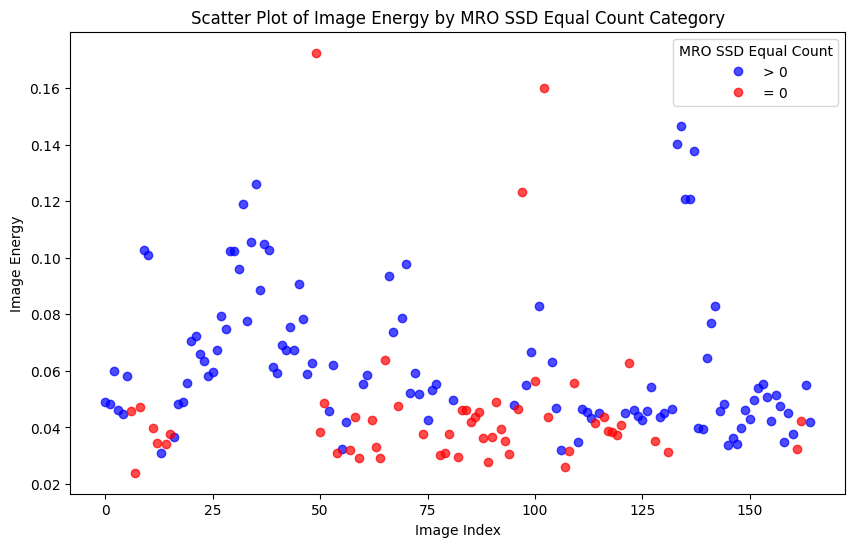
\includegraphics[width=0.9\textwidth]{Figures/Results/sipa_02/energy.png}
    \caption[Image Folder A Energy Analysis on MRO SSD]{Image Folder A Energy Analysis on MRO SSD}
    \label{fig:Image Folder A Energy Analysis on MRO SSD}
\end{figure}




The distribution of Image Energy values for both categories (> 0 and = 0) is quite scattered. This suggests that the distribution of energy values is varied for both cases.

There appears to be a higher density of red points (= 0 category) towards the lower Image Energy values. This suggests that when MRO SSD EQUAL COUNT is zero, the image energy tends to be lower.

There are some apparent outliers in the blue category (gt 0), with significantly higher Image Energy values. This suggests that there might be a few instances with MRO SSD EQUAL COUNT greater than 0 that have unusually high image energy.

There is considerable overlap between the two categories. This indicates that while there might be a general trend (as indicated in points 2 and 3), the MRO SSD EQUAL COUNT value is not a definitive predictor of the Image Energy value.

\newpage

\subsection{Mask Red Function}
% \begin{singlespacing}
\begin{lstlisting}[language=Python, caption=Mask Red Function]

    def mask_red(img):
        """
        Returns an image with only the red pixels from the input image.

        Parameters:
        img (numpy.ndarray): Input image in BGR format.

        Returns:
        numpy.ndarray: Output image with only the red pixels from the input image.

        """
        img_hsv = cv2.cvtColor(img, cv2.COLOR_BGR2HSV)

        # define lower and upper red ranges in HSV
        lower_red1 = np.array([0, 50, 50])
        upper_red1 = np.array([10, 255, 255])
        lower_red2 = np.array([170, 50, 50])
        upper_red2 = np.array([180, 255, 255])

        # create masks with the specified red ranges
        mask1 = cv2.inRange(img_hsv, lower_red1, upper_red1)
        mask2 = cv2.inRange(img_hsv, lower_red2, upper_red2)

        # join the masks
        mask = mask1 + mask2

        # set the output image to zero everywhere except the red mask
        output_img = img.copy()
        output_img[np.where(mask == 0)] = 0

        return output_img


\end{lstlisting}


% \end{singlespacing}

\newpage

\subsection{Mask Green Function}


% \begin{singlespacing}
\begin{lstlisting}[language=Python, caption=Mask Green Function]
    def mask_green(img):
    """
    Returns an image with only the green pixels from the input image.
    
    Parameters:
    img (numpy.ndarray): Input image in BGR format.
    
    Returns:
    numpy.ndarray: Output image with only the green pixels from the input image.
    
    """
    img_hsv = cv2.cvtColor(img, cv2.COLOR_BGR2HSV)
    
    # define range of green color in HSV
    lower_green = np.array([40, 50, 50])
    upper_green = np.array([80, 255, 255])
    
    # create a mask with the specified green range
    mask = cv2.inRange(img_hsv, lower_green, upper_green)
    
    # apply the mask to the image to get the output image
    output_img = cv2.bitwise_and(img, img, mask=mask)
    
    return output_img
    
    
\end{lstlisting}
% \end{singlespacing}




	% Appendix Title


\addtocontents{toc}{\vspace{2em}}  % Add a gap in the Contents, for aesthetics
\backmatter
\end{document}  % The End
%% ----------------------------------------------------------------